\documentclass[paper=a4,fontsize=11pt]{temp} % KOMA-article class
\begin{document}

\newcommand\textbox[1]{%
  \parbox{.333\textwidth}{#1}%
}

\hyphenation{ka-te-go-ri-ze}
\hyphenation{prog-ram-la-ya-bil-mek-tir}

\begin{minipage}{.2\linewidth}
   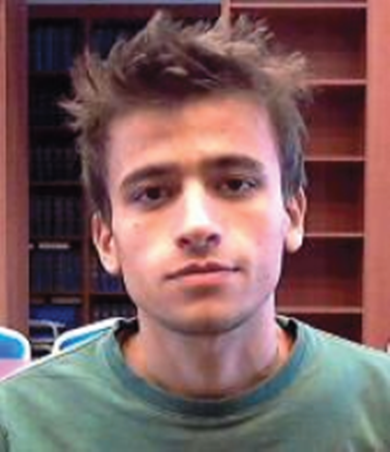
\includegraphics[width=1\textwidth]{photo}
\end{minipage}      
\begin{minipage}{0.7\linewidth}
   \MyName{Fatih Çomak}
   \sepspace

\noindent\textbox{ \hfill}\textbox{\hfil \textbf{
\includegraphics[scale=0.75]{IMG/logo/mail}}\hfil}\textbox{\hfill comakfatihh@gmail.com}

\noindent\textbox{ \hfill}\textbox{\hfil \textbf{
\includegraphics[scale=0.75]{IMG/logo/phone}}\hfil}\textbox{\hfill +90 (534) 310 78 68}

\noindent\textbox{ \hfill}\textbox{\hfil \textbf{
\includegraphics[scale=0.75]{IMG/logo/location}}\hfil}\textbox{\hfill Esenler - İstanbul}

\noindent\textbox{ \hfill}\textbox{\hfil \textbf{
\includegraphics[scale=0.75]{IMG/logo/linkedin}}\hfil}\textbox{\hfill linkedin.com/in/sillyon}

\noindent\textbox{ \hfill}\textbox{\hfil \textbf{
\includegraphics[scale=0.0125]{IMG/logo/github}}\hfil}\textbox{\hfill github.com/Sillyon}

\end{minipage}


\NewPart{Bilgiler}{}
\noindent

\textbox{\textbf{Uyruk \flag{IMG/flag/tr}} \hfill}\textbox{\hfil Türkiye Cumhuriyeti \hfil}\textbox{\hfill}

\textbox{\textbf{Askerlik Durumu} \hfill}\textbox{\hfil Tecilli - 31.12.2021 \hfil}\textbox{\hfill}

\textbox{\textbf{Doğum Tarihi} \hfill}\textbox{\hfil 25.09.1993 \hfil}\textbox{\hfill}

\textbox{\textbf{Doğum Yeri} \hfill}\textbox{\hfil Antalya - Türkiye \hfil}\textbox{\hfill}

\textbox{\textbf{Sürücü Belgesi} \hfill}\textbox{\hfil B, A2 \hfil}


\NewPart{Deneyimler}{}
\indent
\newline
\indent
\workEntry{Xinerji Teknoloji Hizmetleri}{Eylül 2018 - Nisan 2019}{Full Stack Developer, Part-time}{Çok katmanlı mimariye sahip TMAXX isimli lojistik ERP web uygulamasının geliştirilmesinde rol üstlendim. Front-end için Angular, back-end için Java,Hibernate,Spring, server için PostgreSQL kullanıldı.
Ayrıca Flutter Framework, Git kullanımı, Microservices, Docker gibi yenilikçi teknoloji becerileri edindim.} {IMG/xinerji}
\newline\newline
\sepspace

\workEntry{/etcBASE Yazılım ve Bilişim Teknolojileri}{Ağustos 2017 - Eylül 2017}{Yazılımcı, Mesleki Staj}{Başlıca Angular olarak JavaScript frameworkleri ve Spring teknolojileri üzerine araştırmalar yapıldı, dökümantasyonlar tarandı ve karşılaştırmalar yapıldı. TypeScript SPA mimarisi analiz edildi. Bu doğrultuda sunum hazırlandı. Ayrıca Angular CRUD projesi geliştirildi.} {IMG/etcbase}
\newline\newline
\sepspace

\workEntry{Garanti Teknoloji}{Ağustos 2015 - Eylül 2015}{Yazılımcı, Genel Staj}{Mimari ve BT Güvenlik Yönetimi departmanı, Süreç Bilgi Güvenliği ve BT Risk Yönetimi birimi.\\
Web araştırması ve analizi yapıldı. HTML, CSS, (gerektiğinde) JavaScript, SQL, ASP.NET, C\# dilleri öğrenildi; ayrıca ASP.NET Page Life Cycle analiz edildi, client-server Data akışı araştırıldı. Edinilen web mimarisi bilgisi ışığında konsol ve form uygulamaları ile staj projesi olarak da bir demo web uygulaması geliştirildi. Ayrıca müşteri hizmet sistemi ile ilgili beceriler edinildi.}{IMG/garanti}
\sepspace

\NewPart{Eğitim}{}
\indent
\newline
\indent
\EducationEntry{Lisans, Bilgisayar Mühendisliği}{Eylül 2012 - Haziran 2020}{Yıldız Teknik \"{U}niversitesi}{Elektrik-Elektronik Fakültesi} {IMG/ytu_tr}
\newline\newline
\sepspace

\EducationEntry{Isparta Süleyman Demirel Fen Lisesi}{Eylül 2008 - Haziran 2012}{Diploma Notu: 89,3/100}{} {IMG/isdfl}
\sepspace

\NewPart{Yabancı Dil}{}
\indent

\textbox{\textbf{İngilizce \flag{IMG/flag/gb}} \hfill}\textbox{\hfil Profesyonel Çalışma Yetkinliği \hfil}\textbox{\hfill}

\NewPart{Projeler}{}
\indent
\newline
\indent
\workEntry{DevOps Yaklaşımı ile SDLC Dönüşümünde Dockerize Sağlayarak Sürüm Yönetimi}{Ağustos 2019 - Ocak 2020}{Bitirme Tezi}{\textbf{Ekip Arkadaşı:} Selahattin Gürgen\textbf{; Danışman:} Prof.Dr. Oya Kalıpsız \newline
Ulusal Yazılım Mühendisliği Sempozyumu raporları sonucu kurgulanan bu süreçte DevOps yaklaşımı ile uçtan uca Yazılım Geliştirme Yaşam Döngüsü otomasyonu konteynerlaştırılarak semantik versiyon yönetimi sağlandı. Sürüm notunu çıkaran \textbf{Commit Difference Finder} Plugin ve bir script geliştirildi. Git, Jira, Bitbucket, Jenkins, Groovy, Java, Linux Bash, Atlassian SDK kullanıldı. Jira'da task açılmasından ürünün canlıya alınmasına kadar olan süre saniyeler seviyesine indirildi. Esneklik sağlandı.}{IMG/project/devops}

\sepspace

\workEntry{Android Zararlı Yazılımların Word Embeddings ve Makine Öğrenmesi ile Ailelerine Göre Kategorilenmesi}{Ocak 2019 - Haziran 2019}{Akademik Tez Çalışması}{\textbf{Ekip Arkadaşı:} Alibek Erkabayev\textbf{; Danışman:} Arş.Gör. Alper Eğitmen
\newline
Literatür araştırmaları yapıldıktan sonra Android kötü amaçlı yazılımları sınıflandırmak ve kategorize etmek için makine öğrenmesini kullanan, statik opcode analizine dayalı bir yaklaşım sunuldu. Bu yaklaşımda Word Embedding ve Word2Vec yöntemi kullanıldı. Apk DataSet, doğal dil olarak modellendi ve işleme, kelime vektörleri üzerinden gerçeklendi.
C++, Python ile ön-işleme geliştirmesi yazıldı. Veri işlenmesini hızlandırmak ve boyut azaltmak için hashleme yapıldı. 70\%'i train için kullanılan data Weka algoritmalarıyla test edilerek Benign, Malware aileleri kategorilendirildi. Sonuç olarak CBOW için 91,32\%, GloVe için 92,12\% başarı elde edildi.
}{IMG/project/malware}
\sepspace

\workEntry{Kütüphane Otomasyon Sistemi}{Ağustos 2015 - Eylül 2015}{Staj Projesi}{\textbf{Danışman:} Arda Çetinkaya
\newline
Visual Studio ortamında ASP.NET ve C\# tabanlı Web uygulaması Geliştirildi. Bootstrap, jQuery, HTML, CSS, JavaScript, SQL kullanıldı.}{IMG/project/library}
\sepspace

\NewPart{Beceri \& Yetenekler}{}
\hspace{3mm}
\begin{minipage}[t]{0.33\textwidth} 

\begin{tabular}[t]{ l l }
\textbf{Programlama Dilleri}
\end{tabular}

\sepspace

\end{minipage}
%
\begin{minipage}[t]{0.66\textwidth} 



\begin{tabular}{lllllllllll}

\includegraphics[scale=0.035]{IMG/languages/assembly} & \textbf{Assembly} & : & Orta  &  &  & 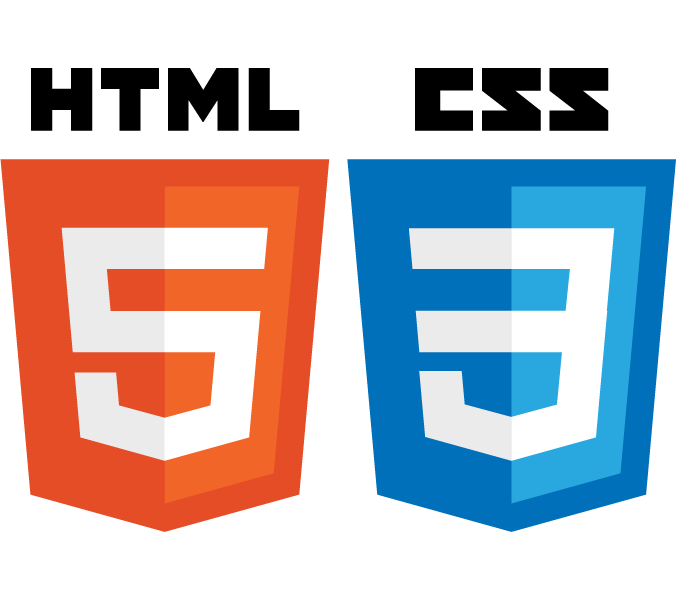
\includegraphics[scale=0.03]{IMG/languages/htmlCss} & \textbf{HTML, CSS}  & : &  & İyi   \\
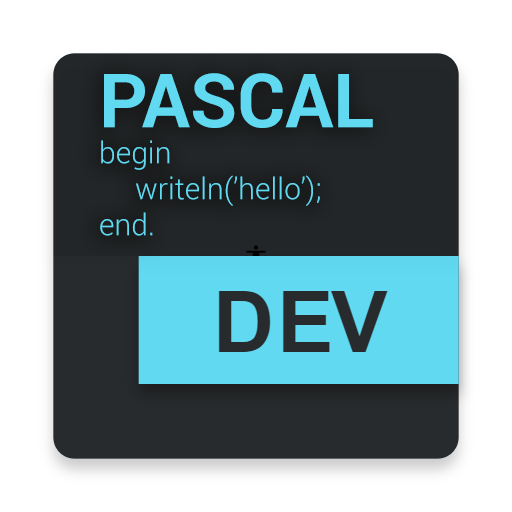
\includegraphics[scale=0.02]{IMG/languages/pascal} & \textbf{Pascal}   & : & Orta  &  &  & 
\includegraphics[scale=0.075]{IMG/languages/javascript} & \textbf{JavaScript} & : &  & Orta  \\

\includegraphics[scale=0.05]{IMG/languages/c} & \textbf{C}        & : & İleri &  &  & 
\includegraphics[scale=0.015]{IMG/languages/aspnet} & \textbf{ASP.NET}    & : &  & Orta  \\

\includegraphics[scale=0.05]{IMG/languages/cplusplus} & \textbf{C++}      & : & Orta  &  &  & 
\includegraphics[scale=0.03]{IMG/languages/prolog} & \textbf{Prolog}     & : &  & Orta  \\

\includegraphics[scale=0.05]{IMG/languages/csharp} & \textbf{C\#}      & : & Orta  &  &  & 
\includegraphics[scale=0.06]{IMG/languages/sql} & \textbf{SQL}        & : &  & İyi   \\

\includegraphics[scale=0.05]{IMG/languages/java} & \textbf{Java}     & : & İyi   &  &  & 
\includegraphics[scale=0.04]{IMG/languages/groovy} & \textbf{Groovy}     & : &  & Temel \\

\includegraphics[scale=0.05]{IMG/languages/python} & \textbf{Python}   & : & Orta  &  &  & 
\includegraphics[scale=0.015]{IMG/languages/matlab} & \textbf{Matlab}     & : &  & Temel
\end{tabular}

\end{minipage} \\\\\\


\begin{minipage}[t]{0.33\textwidth} 

\begin{tabular}[t]{ l l }
\textbf{Yetenekler}
\end{tabular}

\sepspace

\end{minipage}
%
\begin{minipage}[t]{0.66\textwidth} 



\begin{tabular}{llllll}
\textbf{Web Teknolojileri}   & : & 
\includegraphics[scale=0.04]{IMG/tech/angular} Angular, 
\includegraphics[scale=0.04]{IMG/tech/spring}Spring, 
\includegraphics[scale=0.04]{IMG/tech/hibernate} Hibernate                 &  &  &  \\
\textbf{Yapay Zeka}          & : & Makine Öğrenmesi, Uzman Sistemler          &  &  &  \\
\textbf{Programlama}         & : & C (Yapısal), OOP (Nesne Yönelimli)         &  &  &  \\
\textbf{Veritabanı Yönetimi} & : & 
\includegraphics[scale=0.02]{IMG/tech/postgresql} PostgreSQL                                 &  &  &  \\
\textbf{İşletim Sistemleri}  & : & 
\includegraphics[scale=0.03]{IMG/tech/linux} Linux                                      &  &  &  \\
\textbf{Veri Analizi}        & : & Veri Madenciliği, Big Data, Biyoenformatik &  &  & 
\end{tabular}

\end{minipage}


\sepspace

\NewPart{Ek Bilgiler}{}


Öğrenme hevesli ve hızlı adapte olan bir yapıya sahibim. Kariyer hedefim çalıştığım şirketin gelişimine katkıda bulunurken kendimi de geliştirmek; yeteneklerimi ortaya çıkarabildiğim bir firmada zevk alarak yeni projeler programlayabilmektir. Bilgi sahibi olmadığım konularda araştırmalar yapıp kendimi geliştiririm.
\sepspace
\newline
Üniversite döneminde çeşitli mesleki-sosyal aktivitelere(Meetup, seminerler) katıldım.
\sepspace
\newline
\textbf{İlgi Alanlarım : } Doğa sporları, müzik-edebiyat-sinema-fotoğrafçılık, teknoloji-bilgisayar-oyun dünyası.

\end{document}
